\lecture{7}{jeudi 02 avril 2020}
\vspace{-1.2cm}

\section{Digital Targeting}

\subsection{Media buying}

Il existe plein de façons d'acheter des banners publicitaires.

\begin{itemize}
    \item CPM (Cost per thousand): La plus répandue pendant tout un temps, car elle a été la première à apparaitre. Prix pour 1000 impressions. Le but est "l'Awareness".
    \item CPC (Cost per click): Prix par utilisateur qui clique sur le banner. Le but est la "Consideration".
    \item CPL (Cost per lead): Prix par utilisateur qui clique sur le banner et rentre ses données personnelles, générant ainsi un lead. Le but est la "Converstion".
    \item CPA (Cost per action/acquisition): Prix par utilisateur qui achète effectivement le produit. Le but est "l'Acquisition".
    \item CPV (Cost per view): Exemple: pre-roll Youtube.\\
\end{itemize}

\vspace{-0.5cm}
\begin{table}[H]
\begin{tabular}{l|l|l|l|l|l|}
\cline{2-6}
 & \multicolumn{1}{c|}{\textbf{Emplacement}} & \multicolumn{1}{c|}{\textbf{Format}} & \multicolumn{1}{c|}{\textbf{Prix}} & \multicolumn{1}{c|}{\textbf{Inventaire}} & \multicolumn{1}{c|}{\textbf{Temps}} \\ \hline
\multicolumn{1}{|l|}{\textbf{CPM}} & \begin{tabular}[c]{@{}l@{}}Précis\\ (Homepage par exemple)\end{tabular} & \begin{tabular}[c]{@{}l@{}}Premium\\ (fort visible)\end{tabular} & Élevé & Prioritaire & À dates fixes \\ \hline
\multicolumn{1}{|l|}{\textbf{CPC}} & \begin{tabular}[c]{@{}l@{}}Large\\ (sur un style de sites)\end{tabular} & Standard IAB & Normal & Invendus & Date de début et fin \\ \hline
\multicolumn{1}{|l|}{\textbf{CPL}} & Partout & \begin{tabular}[c]{@{}l@{}}Tous les formats\\ disponnibles\end{tabular} & Réduit & \begin{tabular}[c]{@{}l@{}}Beaucoup\\ d'invendus\end{tabular} & Période plus longue \\ \hline
\end{tabular}
\end{table}

\textbf{Budgets}

\begin{itemize}
    \item Display: 40 à 50\% des budgets digitaux chez un annonceur. Petite campagne d'une semaine: 30k euros. Campagne medium: 50 à 80k euros. Campagne large: 100 à 200k euros.
    \item Search: Budget dépend des recherches et de la compétition. 25 à 50\% des budgets digitaux chez un annonceur.
    \item Social: Tendance à la hausse, 30 à 40\% des budgets. Pousser les campagnes sur les réseaux sociaux.
\end{itemize}

\subsection{Real time bidding (RTB)}

Mise aux enchères en temps réel. Des algorithmes travaillent pour relier l'offre et la demande entre les espaces publicitaires disponibles et les demandes d'annonceurs qui veulent communiquer vers certaines cibles. Secteur en évolution constante, qui est disponible pour de plus en plus de touchpoints. On évalue à 54\% les achats digitaux qui se font de manière programmatique.\\

\textbf{Avantages}

\begin{itemize}
    \item Hausse de l'efficacité et du prix ..
    \item Il est possible d'avoir un "engagement" assez fort car on est capables de trouver une audience cible parfaite.
    \item Optimisation en temps réel et "scalable" pour du marketing one-to-one.
    \item Consolidation de l'inventaire.
    \item Statistiques de performance pour une compréhension fine de l'audience.\\
\end{itemize}

\textbf{Définitions clef}

\begin{itemize}
    \item Demand-Side Platform (DSP): Software qui permet d'acheter des placements publicitaires via des enchères.
    \item Supply-Side Platfrom (SSP): Software qui aide les fournisseurs d'emplacements publicitaires à vendre leur inventaire au plus offrant.
    \item Trading Desk: Entreprises focalisées dans l'achat et la vente de publicités au nom de leurs clients, en utilisant plusieurs technologies.
    \item Real-time Bidding: Comme vu plus haut, l'achat et la vente des publicités digitales via des mises aux enchères gérées par des algorithmes, en l'espace d'une milliseconde.\\
\end{itemize}

\subsection{Types de targeting}

\begin{itemize}
    \item Targetting démographique: revenu moyen, âge, genre, origine ethnique, centres d'intérêt, etc.
    \item Targetting géographique
    \item Targetting comportemental: analyse de vos habitudes de navigation
    \item Targetting "look-alike" (sosie): un annonceur va faire un export de sa base de données de client et un algorithme va tirer des conclusions sur les profils des clients actuels pour en trouver des nouveaux.
    \item Retargeting/Remarketing: servir des pubs sur base d'engagements postérieurs du client
    \item Targetting demographique: pub sur base du contexte dans lequel se trouve le potentiel client (e.g. des pubs sportives sur un site de sport)\\
\end{itemize}

\textbf{Types de retargeting}

\begin{itemize}
    \item Product recall: le plus utilisé, on continue à montrer un produit que le client a exploré mais pas acheté
    \item Recommendations: remontrer le produit au client mais avec des recommandations d'autres acheteurs
    \item Cross selling: montrer des nouveaux produits sur base d'achats postérieurs
\end{itemize}

\section{Google Content Strategies}

\begin{figure}[H]
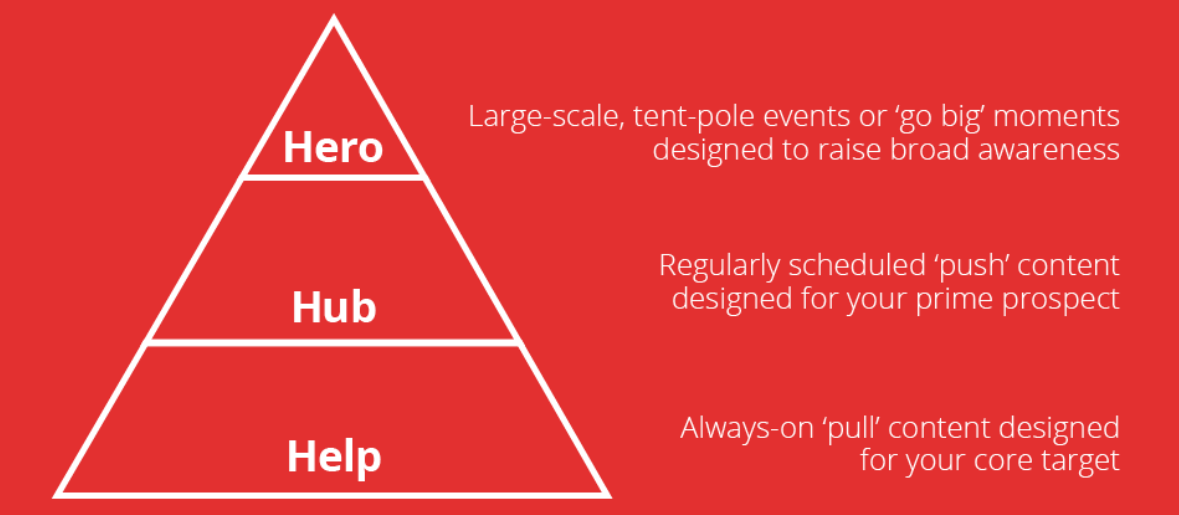
\includegraphics[scale=0.40]{../images/lec7img1}
\end{figure}

Théorie de stratégie de contenu de Google/Youtube, théorie des 3H

\begin{itemize}
    \item Hero: Contenu qui va s'adresser à une cible large, prise de parole quelques fois par an et qui va essayer de diffuser un message lié à la marque pour augmenter l'awareness et l'engagement. Par exemple des campagnes massives, des spots télévisés, des événements majeurs ou des lancements de produits.
    \item Hub: Contenu plus régulier, pour fidéliser le consommateur, pour qu'il revienne souvent. Par exemple du contenu "brandé", des opportunités de sponsorship, des séries vidéo, du contenu de type documentaire ou un "behind the scenes".
    \item Help: Contenu qui va répondre au questionnement du consommateur. Par exemple des videos "how to", des tutoriels, des démonstrations de produit, des témoignages ou des case studes.\\
\end{itemize}
